\documentclass[a4paper, 11pt]{report}

\usepackage[utf8]{inputenc}                                                      
\usepackage[french]{babel}                                                       
\usepackage[T1]{fontenc}  
\usepackage[pdftex]{graphicx}                                                    
\usepackage{url}                                                                 
\usepackage{longtable}
\usepackage[bookmarks, colorlinks=false, pdfborder={0 0 0},
	pdftitle={\texttt{Medicagenda}}, 
	pdfauthor={Knop Florian, Kriwin Paul, Placentino Simon},
	pdfsubject={\texttt{Medicagenda}},           
pdfkeywords={UML, ISO/IEC 19505-1:2012, \texttt{Medicagenda}, Projet, analyse, ESI}]{hyperref}   

\newcommand{\HRule}{\rule{\linewidth}{0.5mm}}    

\begin{document}
\begin{titlepage}
	\begin{center}

		
\includegraphics[keepaspectratio=true,width=0.20\textwidth]{../ressources/logo}\\[1cm]

		\textsc{\LARGE H.E.B. Ecole Superieur d'Informatique}\\[1.5cm]

		\textsc{\Large Laboratoire d'analyse : Projet d'analyse}\\[0.5cm]
		\textsc{\Large Modèle Conceptuel des Traitements}\\[0.5cm]

		\HRule \\[0.4cm]
		{\huge \bfseries Medicagenda \\[0.4cm]}
		\HRule \\[1.5cm]

		\noindent
		\begin{minipage}[t]{0.4\textwidth}
			\begin{flushleft} \large
				\emph{Auteurs:}\\
				Florian \textsc{Knop} \href{mailto:39310@heb.be}{39310@heb.be}\\
				Paul \textsc{Kriwin} \href{mailto:39171@heb.be}{39171@heb.be}\\
				Simon \textsc{Placentino} \href{mailto:39631@heb.be}{39631@heb.be}\
			\end{flushleft}
		\end{minipage}%
		\begin{minipage}[t]{0.4\textwidth}
			\begin{flushright} \large
				\emph{Titulaire du cours:} \\
				Mr.~Nicolas \textsc{Pettiaux}
				\href{mailto:npettiaux@heb.be}{npettiaux@heb.be}
			\end{flushright}
		\end{minipage}

		\vfill

		{\large \today}

	\end{center}
	\clearpage\null\newpage
\end{titlepage}

\tableofcontents

\chapter{Modèle conceptuel des traitements}

\section{Introduction}

\subsection{Objectifs du document}
Ce document présente la décomposition fonctionnelle du projet \texttt{Medicagenda}.
\subsection{Domaine de définition du document}
L'ensemble des sous-systèmes décrits dans le M.C.D. :
\begin{itemize}
	\item SS1 : \texttt{Medicagenda}.
\end{itemize}
\subsection{Définitions, acronymes et abréviations}
\subsection{Références}
\begin{itemize}
	\item[] Etude de cas de l'agenda
		médical\footnote{\href{../Enonce_Travail_Synthese_14-15.pdf}{voir
		étude de cas}}
	\item[] M.C.D. de \texttt{Medicagenda}\footnote{\href{../MCD/MCD.pdf}{voir document M.C.D.}}
\end{itemize}
\newpage
\section{Acteurs}
\subsection{Acteurs externes}
Les acteurs externes au SIA complet du \texttt{Medicagenda} se retrouvent dans le 
diagramme de contexte\footnote{Voir~\ref{dc} Diagramme de contexte} : 
\begin{itemize}
	\item Patient : Personne qui pourra prendre rendez-vous auprès d'un ou
		plusieurs médécin pour une ou plusieurs spécialisation.
\end{itemize}
\subsection{Acteurs internes}
\begin{itemize}
	\item Médecin : Propriétaire de l'agenda pouvant éventuellement être le
		gestionnaire de ce dernier.
\end{itemize}
\subsection{Diagramme des acteurs du SIA}
\begin{figure}[hb]
	\centering
	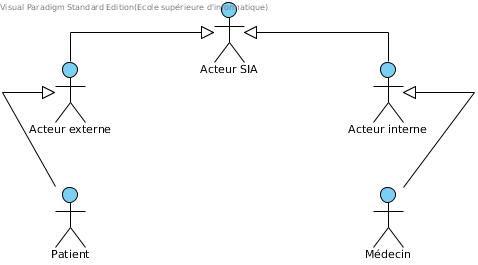
\includegraphics[scale=0.7]{acteurs.jpg}
	\caption{Diagramme des acteurs du SIA}
	\label{fig:acteurs}
\end{figure}
\newpage
\section{Vision globale du SI}
\subsection{\label{dc}Diagramme de contexte}
Ce diagramme présente tout le système informatique du \texttt{Medicagenda} et les acteurs 
externes avec lesquels il est en relation. 
\begin{figure}[hb]
	\centering
	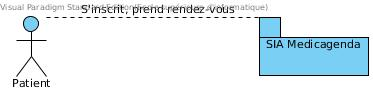
\includegraphics[scale=0.7]{contexte.jpg}
	\caption{Diagramme de contexte}
	\label{fig:contexte}
\end{figure}
\subsection{Diagramme des systèmes}
\begin{figure}[hb]
	\centering
	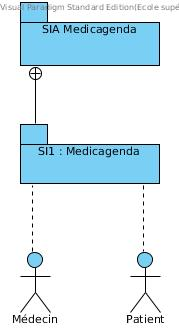
\includegraphics[scale=0.7]{systemes.jpg}
	\caption{Diagramme des systèmes}
	\label{fig:systemes}
\end{figure}
\newpage
\section{Diagramme des sous-sytèmes}
\begin{figure}[hb]
	\centering
	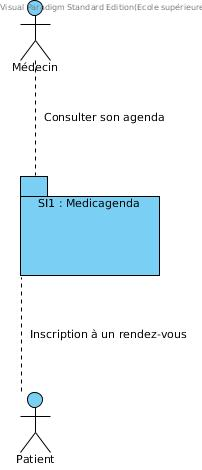
\includegraphics[scale=0.7]{sous-systeme.jpg}
	\caption{Diagramme des sous-systèmes}
	\label{fig:sous-systeme}
\end{figure}
\newpage
\section{Système SI1 : Agenda}
\subsection{Diagramme des Use Cases}
\begin{figure}[hb]
	\centering
	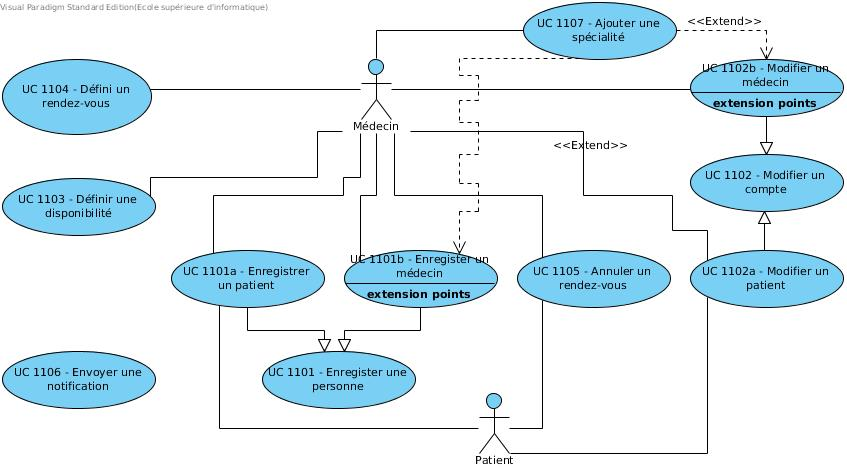
\includegraphics[scale=0.5]{SS1_UC.jpg}
	\caption{Diagramme des Use Cases}
	\label{fig:ss1_uc}
\end{figure}
\subsection{Description des \texttt{U.C.}}
\subsubsection{1101 Enregistrer une personne}
\paragraph{1101a Enregistrer un patient}
Ce \texttt{U.C.} permet créer un nouveau compte pour un patient qui n'en possède pas au
par avant. Ce enregistrement peut se faire :
\begin{itemize}
	\item directement par le patient lui-même,
	\item directement par le médecin lui-même,
	\item directement par le médecin lui-même lors de la prise de rendez-vous.
\end{itemize}
\paragraph{1101b Enregistrer un médecin}
Ce \texttt{U.C.} permet créer un nouveau compte pour un médecin qui n'en possède pas au
par avant. Ce enregistrement peut se faire :
\begin{itemize}
	\item directement par le médecin lui-même,
	\item par un organisme externe déployant le système (tel que l'INAMI).
\end{itemize}

L'enregistrement d'un nouveau médecin peut entrainer 
\begin{itemize}
	\item l'enregistrement de	spécialités associées à ce dernier ne se trouvant pas déjà dans la 
		BDD\footnote{Base De Données}.
	\item la création d'un nouveau calendrier.
\end{itemize}
Ce \texttt{U.C.} peut donc faire appel au \texttt{U.C. 1107}.
\subsubsection{1102 Modifier un compte}

\paragraph{1102a Modifier un patient}
Ce \texttt{U.C.} permet de modifier les données d'un compte. Cette modification
peut se faire :
\begin{itemize}
	\item par le médecin directement n'intervenant que sur un certain niveau de
		données,
	\item par le patient directement n'intervenant que sur un certain niveau de
		données.
\end{itemize}

Certaines modifications de données, telles que l'annulation d'un rendez-vous par
l'un ou par l'autre, doivent être notifiée.

Le patient peut ainsi s'inscrire à un rendez-vous selon les disponibilités
proposées par le médecin.
\paragraph{1102b Modifier un médecin}
Ce \texttt{U.C.} permet, uniquement au \textbf{médecin}(on éventuellement à un
service externe tel que l'INAMI) de modifier son compte.

Il peut faire appel aux 
\begin{itemize}
	\item \texttt{~U.C. 1103} 
	\item \texttt{~U.C. 1104} 
	\item \texttt{~U.C. 1105}
	\item \texttt{~U.C. 1107}
\end{itemize}

\subsubsection{\label{1103}1103 Définir une disponibilité}
Ce \texttt{U.C.} permet a un médecin de définir une plage de disponibilité dans
un jour du calendrier. Il permet, aussi, de redéfinir une disponibilité après
l'annulation d'un rendez-vous.
\subsubsection{\label{1104}1104 Définir un rendez-vous}
Ce \texttt{U.C.} permet à un patient de définir un rendez-vous selon le
calendrier d'un médecin en se basant sur l'ensemble de ses disponibilités. 
Ce \texttt{U.C.} peut aussi être effectué par un médecin pour le compte d'un
patient directement si un nouveau rendez-vous doit être fixé.

Le rendez-vous enclenchera l'ajout d'un entrée dans le mécanisme des
notifications.
\subsubsection{\label{1105}1105 Annuler un rendez-vous}
Ce \texttt{U.C.} permet a une disponibilité de l'agenda d'être à nouveau
disponible. L'annulation peut être faite par le patient ou par le médecin. 
\subsubsection{\label{1106}1106 Envoyer une notification}
Ce \texttt{U.C.} \textbf{automatisé} envoie des notifications aux patients ayant
un rendez-vous. Celle-ci sera envoyée à l'heure définie par le médecin, si le
patient n'a pas annulé avant, la consultation lui sera facturée.
\subsubsection{\label{1107}1107 Ajouter une spécialité}
Ce \texttt{U.C.} permet de rajouter des spécialités dans la base de données et
uniquement par un médecin. Cet ajout doit passer par un organisme, tel que
l'INAMI, pouvant le confirmer.
\newpage
\subsection{Matrice CRUD}

Pour la lisibilité de la matrice, cette dernière a été séparé en deux tableaux.
Seuls les UC ayant une action avec une des classes du tableau apparaissent.

\begin{center}
	\begin{longtable}{|p{1.5cm}|p{1.5cm}|p{1.5cm}|p{1.5cm}|p{1.5cm}|}
		\hline
		& Compte & Compte Mèdecin & Compte Patient & Spécialité \\
		\hline
		UC1101a & C & / & C & / \\
		\hline
		UC1101b & C & C & / & R \\
		\hline
		UC1102  & U & / & U & / \\
		\hline
		UC1105  & R & R & R & R \\
		\hline
		UC1106 & R & R & R & R \\
		\hline

	\end{longtable}
\end{center}

\begin{center}
	\begin{longtable}{|p{2.2cm}|p{2.2cm}|p{2.2cm}|p{2.2cm}|}
		\hline
		& Evènement & Rendez-vous & Disponnibilité  \\
		\hline
		UC1103 & C & R & C \\
		\hline 
		UC1104 & C & C & R \\
		\hline
		UC1105 & U & U & / \\
		\hline
		UC1106 & R & R & / \\
		\hline

	\end{longtable}
\end{center}
\end{document}
